\documentclass[12pt,answers]{exam}

\usepackage[margin=0.5in]{geometry}
\usepackage{amsmath}
\usepackage{tikz}
\usepackage{hyperref}
\usepackage{multicol}



\newcommand{\ds}{\displaystyle}

\begin{document}
\pagestyle{empty}
\subsubsection*{Practice Final Exam - Math 140 }
\begin{questions}

\question Find the intervals of increase/decrease for $f(x) = \frac{1}{4}x^4 - \frac{1}{3}x^3 - 6 x^{2}$.
\begin{solution}
$f'(x) = x^3 - x^2 - 12x$ which factors as $x(x-4)(x+3)$.  Therefore decreasing on $(-\infty,-3)$ and $(0,4)$, increasing on $(-3,0)$ and $(4,\infty)$.
\end{solution}
\vfill

\question Use the logarithm rules to simplify, then differentiate $\ds y= \ln \left( \frac{x}{(x+4)^2} \right)$.  
\begin{solution}
$\ds y = \ln x - 2 \ln (x+4)$, therefore $\ds y' = \frac{1}{x} - \frac{2}{x+4}$. 
\end{solution}
\vfill


\question Find a formula for the linear function $f(x)$ with $f(0) = -1$ and $f(3) = 5$.  
\begin{solution}
The slope is 2 and the y-intercept is $-1$, so the line is $f(x) = 2x-1$.
\end{solution}
\vfill


\question The graph of a function $y = g(x)$ is shown.  Use the graph to find the following.

\noindent
\begin{minipage}{0.4\textwidth}
\begin{parts}
\part What are the roots of $g(x)$? \\ 
\begin{solution}
The graph hits the x-axis at $-2$, 0, and 1. 
\end{solution}
\vspace*{0.7in}

\part What is $g(-1)$?  \\ 
\begin{solution}
It looks like $g(-1) = 2$. 
\end{solution}
\vspace*{0.7in}

\part Is $g'(-1)$ positive, negative, or zero? \\

\begin{solution}
It is negative.
\end{solution}
\vspace*{0.7in}

%\part What is $g(g(-1))$? \\ \\ 

\end{parts}
\end{minipage}
\hfill
\begin{minipage}{0.6\textwidth}
\begin{center}
\begin{tikzpicture}[xscale=0.7,yscale=0.7]
%\draw[gray!60] (-3.3,-3.3) grid (3.3,3.3);
\draw[very thick,->] (-3.5,0) -- (3.5,0) node[below right,scale=0.6] {$x$};
\draw[very thick,->] (0,-3.5) -- (0,3.5) node[above left,scale=0.6] {$y$};
\draw[very thick,color=blue] plot[domain=-2.4:1.6,samples=100] function {x**3+x**2-2*x} node[right] {$g(x)$};
\foreach \x in {-3,-2,-1,1,2,3} {
  \draw (\x,0.1) -- +(0,-0.2) node[below,scale=0.5] {\x};
  \draw (0.1,\x) -- +(-0.2,0) node[left,scale=0.5] {\x};
}
\end{tikzpicture}
\end{center}
\end{minipage}
\newpage

\question Solve $\ds \frac{1}{x} - \frac{2}{x+4} = 0.$
\begin{solution}
With common denominators you get: $\ds \frac{x+4 - 2x}{x(x+4)} = \frac{4-x}{x(x+4)} = 0$, so the solution is $x = 4$. 
\end{solution}
\vfill


\question Find the following derivatives.
\begin{parts}
\begin{multicols}{2}
\part $\dfrac{d}{dx} x^{1/5}$ 
\begin{solution}
Power rule: 
$$\tfrac{1}{5} x^{-4/5}$$  
\end{solution}
\part $\dfrac{d}{dx} e^{(x^2 + 3x)}$
\begin{solution}
Chain rule: $$(2x+3) e^{(x^2 + 3x)}$$
\end{solution}
\end{multicols}
\vfill

\begin{multicols}{2}
\part $\dfrac{d}{dx} \dfrac{x+5}{x^2 - 4}$
\begin{solution}
Quotient rule: 
$$\dfrac{(x^2-4)-(x+5)(2x)}{(x^2-4)^2}$$
\end{solution}
\part $\dfrac{d}{dx} x^2 e^x$
\begin{solution}
Product rule:
$$2x e^x + x^2 e^x$$
\end{solution}
\end{multicols}
\vfill
\end{parts}

\question Find the $(x,y)$ coordinates of the local max of $f(x,y) = 9 - x^2 - y^2 + 6y$. 
\begin{solution}
Set the partial derivatives equal to zero and solve:
$$f_x = -2x = 0$$
$$f_y = -2y + 6 = 0$$
So $x = 0$ and $y = 3$. 
To check that this is a max, find the 2nd partial derivatives and calculate the determinant $f_{xx} f_{yy} - (f_{xy})^2$. 
$$f_{xx} = -2, ~~~~ f_{yy} = -2, ~~~~ f_{xy}  = 0, $$
So $D = 4$ and therefore $(0,3)$ is a local max by the second derivative test.
\end{solution}
\vfill

\newpage


\question What is the slope of the tangent line to $h(x) = \tfrac{1}{3}x^3 - 3x^2 + 5x$ at the point $(3,-3)$?
\begin{solution}
The derivative is $h'(x) = x^2 - 6x + 5$.  Plug in $x=3$ to get $9 - 18 + 5 = -4$ as the slope of the tangent line. 
\end{solution}
\vfill

\question Find the differential of $y = e^{x}$ at $x = 0$ when $dx = 0.1$ and use it to estimate the value of $e^{0.1}$. 
\begin{solution}
$$dy = e^x dx$$
Substituting $x = 0$ and $dx = 0.1$, we get $dy = 0.1$.  We also know that when $x=0$, $y = e^0 = 1$, so we adjust that by adding the $dy$ to get 
$$e^{0.1} \approx 1.1.$$
\end{solution}

%\begin{flushright}
%\begin{tikzpicture}[scale=0.7]
%\draw[very thick,->] (-0.25,0) -- (5.25,0) node[below right] {$x$};
%\draw[very thick,->] (0,-0.25) -- (0,3.25) node[above left] {$y$};
%\foreach \x in {1,2,3,4,5} {
%  \draw (\x,0.1) -- +(0,-0.2) node[below,scale=0.5] {\x};
%}
%\foreach \y in {1,2,3} {
%  \draw (\y,0.1) -- +(0,-0.2) node[left,scale=0.5] {\y};
%}
%\draw[very thick,color=blue] plot[domain=0:5.25,samples=100] function {x**0.5} node[right] {$f(x)$};
%\end{tikzpicture}
%\end{flushright}
\vfill


\question Simplify $(\sqrt{2} + \sqrt{50})^2$. \textit{Remember: Powers don't distribute to terms!}
\begin{solution}
FOIL: $(\sqrt{2} + \sqrt{50})(\sqrt{2} + \sqrt{50}) = 2 + 10 + 10 + 50 = 72$. 
\end{solution}
\vfill

\question Find the absolute maximum and minimum $y$-values of the function $y = x + \dfrac{100}{x}$ on the interval $[5,25]$.  
\begin{solution}
$y' = 1 - 100 x^{-2}$. Therefore $x = 10$ is a critical point.  So we calculate the y-values at the critical point and the endpoints:

\begin{tabular}{c|c}
$x$ & $y$ \\ \hline
5 & 25 \\
10 & 20 \\ 
25 & 29 
\end{tabular}

Therefore the absolute max is at $(25, 29)$ and the absolute min is at $(10,20)$.
\end{solution}
\vfill

\newpage

\question Suppose that the population of a town is growing by 5\% per year and the current population is 10{,}000, so the formula for the population after $t$ years is 
$$P(t) = 10{,}000 (1.05)^t.$$  
How long will it be until the population of the town reaches 30,000 people?  It is okay to write your answer as a formula using logarithms. 
\begin{solution}
Solving $10{,}000(1.05)^t = 30{,}000$ is the same as solving $(1.05)^t = 3$.  Take the natural-log of both sides, then solve for $t$ to get 
$$t = \dfrac{\ln 3}{\ln 1.05}.$$
\end{solution}
\vfill

\question Solve $2 e^{5x} = 64$. 
\begin{solution}
$5x = \ln 32$, so $x = \frac{1}{5} \ln 32 = \ln 2$. 
\end{solution}
\vfill

\question A fruit importer will sell $q(p) = 800 - 20p$ boxes of fruit when the price of a box is $p$ dollars. What price would maximize the fruit importer's revenue? 
\begin{solution}
$R = 800p - 20p^2$ so $R' = 800 - 40 p = 0$ when $ p = 800/40 = 20$.  Since the second derivative is $-40$, this is a max. 
\end{solution}
\vfill


\question Calculate the following logarithms.
\begin{multicols}{2}
\begin{parts}
\part $\ds \log_3(9)$ 
\begin{solution}
2 \\
\end{solution} 
\part $\ds \log_2 \left( \frac{8}{\sqrt{2}} \right)$
\begin{solution}
$3-0.5 = 2.5$
\end{solution}
\end{parts}
\end{multicols}
\vfill

\newpage

\question Find the partial derivatives (both $f_x$ and $f_y$) for $f(x,y) = x^2 + y^4 + 2xy^3$.
\begin{solution}
$f_x = 2x + 2y^3$ and $f_y = 4y^3 + 6xy^2$.
\end{solution}
\vfill

\question The production level at a factory is $Q(x,y) = 40x^{0.25} y^{0.75}$ where $x$ is hours of labor and $y$ is capital expenditure.  Find the partial derivatives of $Q$ when $x = 100$ and $y = 100$.  %Then use the formula $\ds \Delta Q \approx \frac{\partial Q}{\partial x} \Delta x + \frac{\partial Q}{\partial y} \Delta y$ to estimate how much production would increase if the factory reduced labor by 2 units and increased capital by 1 unit.  
\begin{solution}
$Q_x = 10 x^{-0.75}y^{0.75}$ and $Q_y = 30 x^{0.25} y^{-0.25}$. Plugging in 100 for $x$ and $y$, we get $Q_x = 10$ units of output per hour of labor and $Q_y = 30$ units of output per dollar of capital expenditure.%, so dropping labor 2 units would decrease output by 20, but increasing capital by 1 would increase output by 30, so the net change would be output increases by 10. 
\end{solution}
\vfill 

\question A box with a square bottom and an open top needs to have exactly 4 cubic feet of volume.  Find the dimensions of the box with the smallest possible surface area.  Recall that the volume of a box is $V = x^2 y$ where $x$ is the length and width and $y$ is the height.  The surface area is $S = 4xy + x^2$.  
\begin{solution}
Substituting $y = 4/x^2$ into $S$, we get $S = 16/x + x^2$.  So $S' = -16/x^2 + 2x = 0$ when $x = 2$. Then $y = 1$.  And that is a minimum since $S'' = 32/x^3 + 2$ which is positive.  

\textbf{Solution using Lagrange multipliers} \\
Constraint: $V = x^2 y = 4$
Objective: $S = 4xy + x^2$. 
\end{solution}
\vfill
\vfill

\end{questions}

%\newpage
%\section*{Formula Sheet}
%
%\begin{description}
%\item[Quadratic Formula] $$\ds x = \frac{-b \pm \sqrt{b^2 - 4ac}}{2a}.$$
%
%\item[Point-Slope Formula] $$y-y_0 = m (x-x_0)$$
%
%\item[Linear Approximation Function] $$L(x) = f(x_0) + f'(x_0) (x-x_0)$$
%
%\item[Derivatives of Exponentials] $$\dfrac{d}{dx} a^x = a^x \ln a$$
%
%\item[Derivative of Natural Logarithm] $$\dfrac{d}{dx} \ln x = \dfrac{1}{x}$$
%
%\item[Price Elasticity of Demand] $$E = \left| \frac{p \, Q'}{Q} \right|$$
%\end{description}
%
\end{document}


\color{gray}
%%% Midterm 1 Questions



\question Simplify $\ds  \frac{30 a}{5} \cdot \sqrt{\frac{b^2}{9a^6}}$
\begin{solution}
$$\frac{2b}{a^2}$$
\end{solution}
\vfill



\hrule



%\question In order to produce $x$ widgets, a company must invest \$200 up front, and then each widget costs \$5 to make.  What is the total cost $C(x)$ of the widgets the company makes as a function of the number of widgets produced $x$?  
%\begin{solution}
%$$C(x) = 200 + 5x$$
%\end{solution}
%\vfill
%\hrule
\newpage

\question Suppose that a ball is thrown up in the air over the head of a person standing at the origin. The ball follows a parabolic trajectory with $h(x) = -\frac{1}{2} x^2 + 4x + 10$ where $h$ is the height of the ball above the ground and $x$ is the horizontal position of the ball relative to the person at the origin.  Draw a graph of the path the ball travels. Be sure to label the $x$ and $y$-coordinates of the vertex (where the ball is highest in the air) and the $x$-coordinates where the ball starts and finishes its path. 
\begin{flushright}
\begin{tikzpicture}
\draw[very thick,<->] (-3,0) -- (3,0);
\draw[very thick,<->] (0,-1) -- (0,3);
\end{tikzpicture}
\end{flushright}
\begin{solution}
\end{solution}
\vfill
\hrule
\color{black}

\question Graph the function $f(x) = \ds \sqrt{x+4}$. Be sure to label any points where the function crosses the $x$ or $y$-axis.
\begin{flushright}
\begin{tikzpicture}
\draw[very thick,<->] (-3,0) -- (3,0);
\draw[very thick,<->] (0,-2) -- (0,2);
\end{tikzpicture}
\end{flushright}
\begin{solution}
\end{solution}
\vfill
\hrule


\question Simplify by factoring $\ds \frac{x^2-5x+6}{4x-8}$.
\begin{solution}
$$\frac{x^2-5x+6}{4x^2-8} = \frac{(x-2)(x-3)}{4(x-2)} = \frac{x-3}{4}$$
\end{solution}
\vfill
\vfill
\vfill
\hrule

\question Simplify $(\sqrt{2} + \sqrt{50})^2$. 
\begin{solution}
$$(\sqrt{2}+\sqrt{50})^2 = 2 + 2 \sqrt{2}\sqrt{50} + 50 = 52 + 2 \sqrt{100} = 72$$
\end{solution}
\vfill
\vfill
\vfill
\hrule

\newpage
\question Suppose that $f(x) = 4x-1$ and $g(x) = \dfrac{1}{x+2}$.  Calculate the following.
\begin{parts}
\part $g(f(1))$ 
\vfill
\part $f(g(0))$ 
\vfill
\end{parts}
\begin{solution}
\end{solution}
\hrule


\question Doctors are testing the effectiveness of a new pain medicine.  They are trying to find a function $P(d)$ to predict a patients pain level (on a scale from 0 to 10) as a function of the dose $d$ that the patient receives (in milligrams).  If $P(5) = 7$, what does that mean about dose and pain levels? Write a complete sentence to explain. 
\vfill
\vfill
\hrule

\question Continuing the last problem.  Over time, the dose remaining in a patients body will decrease, so $d$ is a function of time $t$ (measured in hours).  That is $d = d(t)$. Which of the following would be the right way to predict a patient's pain level 6 hours after taking a dose of pain killer?  (Circle one.) \\

\begin{choices}
\choice Calculate $d(P(6))$.  \\
\choice Solve $6 = P(d(t))$.   \\
\choice Solve $6 = d(P(t))$.   \\
\choice Calculate $P(d(6))$. \\
\end{choices} 
~\\ 
~\\
\hrule

\newpage
\question Simplify the following as much as possible. 
\begin{parts}
\part $(5x^3)^2 x^7$ 
\vfill

\part $\dfrac{6 x^{-4}}{2 x^{-1}}$ 
\vfill
\end{parts} 
\hrule 



\question  If a gas station sets the price of gas at \$2 per gallon, they will sell 18,000 gallons of gas.  Assume that the quantity of gas sold is a linear function and for every dollar the price increases, the quantity sold decreases by 9,000 gallons, so $Q(p) = 18000 - 9000(p-2)$.  What are the slope and $y$-intercept for this linear function?
\vfill
\vfill
\hrule


\question Continuing the last problem.  Revenue is price times quantity sold.  Find a formula for the revenue $R$ at this gas station as a function of price $p$. Then graph the revenue function and find the price where revenue is the highest.
\begin{flushright}
\begin{tikzpicture}
\draw[very thick,<->] (-3,0) -- (3,0);
\draw[very thick,<->] (0,-2) -- (0,2);
\end{tikzpicture}
\end{flushright}
\vfill
\hrule


\newpage
\question Factor the equation $Ax + B^2x = 1$ and solve for $x$. 
\vfill
\hrule

\question Simplify the following as much as possible. $\ds \frac{~\dfrac{1}{x+h} - \dfrac{1}{x}~}{h}$.
\vfill
\hrule

%%% Midterm 2 Questions 


\question[5] Solve $x^2 + 2x - 8 > 0$.
\vfill 

\hrule 

\fullwidth{Let $g(x) = \dfrac{3x-6}{x^3 - 2x^2}$ (shown in the graph below).}
\question[5]  There are two $x$-values where $g(x)$ is discontinuous.  What are they?
\begin{center}
\begin{tikzpicture}[scale=0.75]
\draw[very thick,->] (-4,0) -- (4,0) node[below right,scale=0.6] {$x$};
\draw[very thick,->] (0,-1) -- (0,4) node[above left, scale=0.6] {$y$};
\draw[very thick,color=blue,<->] plot[domain=0.85:3.9,samples=400] function {(3*x-6)/(x**3-2*x**2)};
\draw[very thick,color=blue,<->] plot[domain=-3.9:-0.85,samples=400] function {(3*x-6)/(x**3-2*x**2)};
\filldraw[draw=blue,fill=white,thick] (2,0.75) circle (0.075);
\end{tikzpicture}
\end{center}

\begin{multicols}{2}
\question[5] Find $\ds \lim_{x \rightarrow 0} \, \dfrac{3x-6}{~x^3 - 2x^2~} $.

\question[5] Find $\ds \lim_{x \rightarrow 2} \, \dfrac{3x-6}{~x^3 - 2x^2~} $.
\end{multicols}
\vfill
\hrule


\newpage


\question[5] Find the derivative of $\ds y = 5x^6 - 4 x + 3$. 
\vfill

\hrule






\question[5] Solve $\ds \frac{4}{x} > x+3$.  
\vfill
\hrule


\newpage
\question[5] Find $\ds \frac{d}{dx} \sqrt{x+x^2}$.
\vfill

\hrule



\hrule

\question[5] Where is the function $h(x) = \tfrac{1}{3}x^3 - 3x^2 + 5x$ concave down? 
\vfill
\hrule

\question[5] Let $f(x) = x^3 - 6x^2 + x - 5$.  Find the equation of the tangent line to $f(x)$ when $x = 0$.  
\begin{flushright}
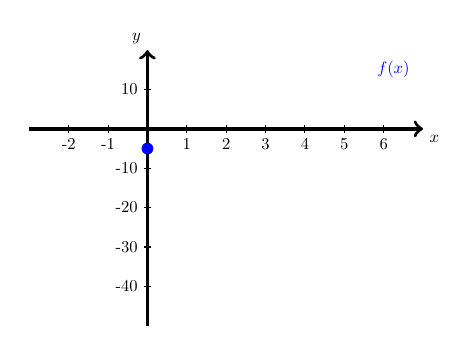
\begin{tikzpicture}[scale=0.5]
\draw[very thick,->] (-3,0) -- (7,0) node[below right,scale=0.6] {$x$};
\draw[very thick,->] (0,-5) -- (0,2) node[above left, scale=0.6] {$y$};
\draw[very thick,color=blue] plot[domain=-2.1:6.2,samples=400] function {(x**3-6*(x**2)+x-5)/10};
\fill[blue] (0,-0.5) circle (0.15);
\foreach \y in {-4,-3,-2,-1,1} {
  \draw (0.1,\y) -- (-0.1,\y) node[left,scale=0.6] {\y0};
}
\foreach \x in {-2,-1,1,2,3,4,5,6} {
  \draw (\x,0.1) -- (\x,-0.1) node[below,scale=0.6] {\x};
}
\draw[blue] (6.25,1.5) node[scale=0.6] {$f(x)$};

\end{tikzpicture}
\end{flushright}

\hrule





\newpage

%\question[5] According to the theory of special relativity, if a spaceship with rest mass of 1,000 kg travels with velocity $v$ measured as a fraction of the speed of light, then the relativistic mass of the spaceship is a function of $v$ given by the formula:
%$$m(v) = 1000(1 - v^2)^{-1/2}$$ 
%Use the chain rule to find out how fast the spaceship's mass is increasing with respect to time when the velocity of the spaceship is 0.6 times the speed of light and is increasing by 0.01 every day. 
%
%\vfill
%
%\hrule


\question[5] The owner of a cake shop estimates that the total cost of making $x$ cakes in a day is 
$$C(x) = 100 + 2x + \tfrac{1}{10}x^2.$$  
Find the derivative of $C(x)$ and use it to estimate the marginal cost of making an extra cake if the shop typically makes 20 cakes per day.  
\vfill

\hrule

\question[5] Find $\ds \lim_{h \rightarrow 0} \frac{h^3 + 6 h^2 + 12 h}{h}$.
\vfill

\hrule

\question[5] Calculate the following limits:
\begin{parts}
\begin{multicols}{2}
\part $\ds \lim_{x \rightarrow 2^+} \frac{1}{2-x}$  
\part $\ds \lim_{x \rightarrow 4} \frac{4-x}{3}$
\end{multicols}
\end{parts}
\vfill

\hrule 

\question[5] According to the theory of special relativity, if a spaceship with rest mass of 1,000 kg travels with velocity $v$ measured as a fraction of the speed of light, then the relativistic mass of the spaceship is a function of $v$ given by the formula: $m(v) = 1000(1 - v^2)^{-1/2}$.
Find $\dfrac{dm}{dv}$.
\vfill
\hrule


%%% Midterm 3 Questions
\question[10] Find the absolute max and min for $f(x) = 2x(x-4)$ on the interval $[0,5]$.
\vfill 
 

\question[10] Find the intervals of increase \& decrease for the function $g(x) = \frac{1}{5} x^{5} - 2 x^{4} + 5 x^{3}$.
\vfill



\question[10] Suppose that the population of a town is growing by 5\% per year and the current population is 4000.  How long will it be until the population of the town reaches 6000 people?  It is okay to write your answer as a formula using logarithms. 
\vfill


\newpage
\question[10] Find the differential of $y = e^{x}$ at $x = 0$ when $dx = 0.1$ and use it to estimate the value of $e^{0.1}$. 
\begin{solution}
$$dy = e^x dx$$
Substituting $x = 0$ and $dx = 0.1$, we get $dy = 0.1$.  We also know that when $x=0$, $y = e^0 = 1$, so we adjust that by adding the $dy$ to get 
$$e^{0.1} \approx 1.1.$$
\end{solution}
\vfill
\vfill
\vfill


\question[10] A rectangle has bottom left corner at the origin and top right corner on the line $y = 6-2x$.  Find the dimensions of the rectangle with largest area that fits under the line $y = 6 - 2x$ as shown below. 
\begin{flushright}
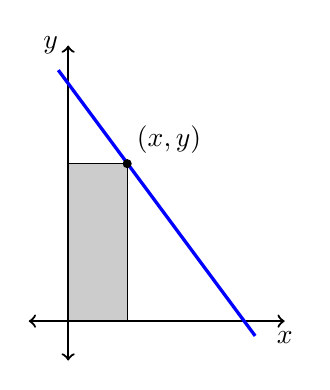
\begin{tikzpicture}[scale=0.5]
\filldraw[fill=gray!40] (0,0) rectangle (1.5,4);
\draw[thick,<->] (-1,0) -- (5.5,0) node[below] {$x$};
\draw[thick,<->] (0,-1) -- (0,7) node[left] {$y$};
\draw[very thick,color=blue] (-0.25,6.375) -- (4.75,-0.375);
\filldraw (1.5,4) circle (0.1) node[above right] {$(x,y)$};
\end{tikzpicture}
\end{flushright}
\vfill
\vfill





\question[10] Calculate the following derivatives.
\begin{parts}
\begin{multicols}{2}
\part $\dfrac{d}{dx} e^{4x^2}$ 
\part $\dfrac{d}{dx} (x^2 + x) \cdot e^x$
\end{multicols}
\end{parts}
\vfill
\vfill
\vfill

\newpage
\question[10] Calculate the exact values of the following logarithms.
\begin{parts}
\begin{multicols}{2}
\part $\log_3(9)$
\part $\log_4(\frac{1}{16})$ 
\end{multicols}
\vfill

\begin{multicols}{2}
\part $\log_5(\sqrt{5})$
\part $\ln(1)$ 
\end{multicols}
\end{parts}
\vfill


\question[10] A farmer has a crop of rare fruit.  If the farmer harvests the fruit now, he will get 10 crates of fruit.  For every day he waits, the number of crates he can harvest will decrease by 1.  At the same time, the price of the fruit is currently only \$10 per crate, but will increase by \$5 every day that the farmer waits.  Find a formula for the revenue as a function of the number of days the farmer waits, then use calculus to find the optimal number of days the farmer should wait to maximize his revenue. 
\vfill
\vfill
\vfill





\question[10] Solve $4e^{2x}  = 12$. It is okay to express your answer using logarithms.
\vfill
\vfill
\vfill

\newpage


\question[10] Find the derivative of $\ds f(x) = \ln\left( \frac{x^2}{x-1} \right)$. Hint: Use the properties of logarithms to simplify $f(x)$ before taking the derivative.
\vfill

\question[10] Let $f(x) = x^2 + e^x$.  Find $f'(x)$ and $f''(x)$.  Then use $f''(x)$ to write a sentence that explains why the critical point at $x = -0.352$ must be a minimum.  

\begin{flushright}
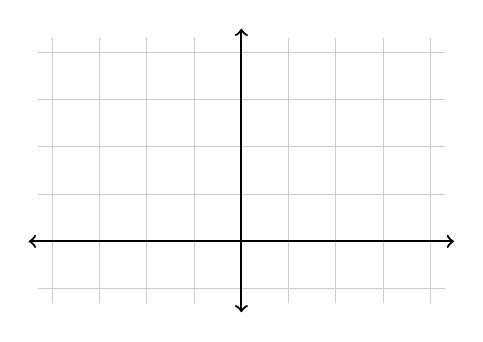
\begin{tikzpicture}[scale=0.6]
\draw[thin,gray!40] (-4.3,-1.3) grid (4.3,4.3);
\draw[thick,<->] (-4.5,0) -- (4.5,0);
\draw[thick,<->] (0,-1.5) -- (0,4.5);
\draw[very thick,color=blue] plot[domain=-2:1.1,samples=400] function {x**2+exp(x)};
\end{tikzpicture}
\end{flushright}
\vfill

\end{questions}
\newpage

\section*{Formula Sheet}

\begin{description}
\item[Quadratic Formula] $$\ds x = \frac{-b \pm \sqrt{b^2 - 4ac}}{2a}.$$

\item[Point-Slope Formula] $$y-y_0 = m (x-x_0)$$

\item[Linear Approximation Function] $$L(x) = f(x_0) + f'(x_0) (x-x_0)$$

\item[Derivatives of Exponentials] $$\dfrac{d}{dx} a^x = a^x \ln a$$

\item[Derivative of Natural Logarithm] $$\dfrac{d}{dx} \ln x = \dfrac{1}{x}$$

\item[Price Elasticity of Demand] $$E = \left| \frac{p \, Q'}{Q} \right|$$
\end{description}

\end{document}
